\documentclass[10pt,twocolumn]{article}
\usepackage[margin=1in]{geometry}
\usepackage{amsmath,amssymb}
\usepackage{booktabs}
\usepackage{graphicx}
\usepackage{hyperref}
\usepackage{microtype}
\usepackage{parskip}
\usepackage{xurl}
\setlength{\emergencystretch}{3em}

\title{\textbf{Do LLMs Play Nash?}\\
       \large Strategic Behavior of Language Models}
\author{David Hung\\
        \small CSCE 631 --- Summer I 2026, Texas A\&M University\\
        \small \texttt{david\_hung@tamu.edu}}
\date{}

\begin{document}
\maketitle

%% ─────────────────────────────────────────────
\section{Introduction}
%% ─────────────────────────────────────────────

Large language models (LLMs) are increasingly deployed as autonomous decision-making
agents in negotiation, resource allocation, and multi-agent systems.
A natural question from the perspective of game theory is whether these models behave
\emph{strategically}: when placed in a well-defined game, do their action choices
approximate Nash equilibrium (NE) strategies?

A Nash equilibrium is a strategy profile from which no player can profitably deviate
unilaterally~\cite{nash1950equilibrium}.
If an LLM's strategy is exploitable---i.e., an opponent can earn positive surplus
by best-responding to it---then the model is not playing Nash.
Measuring this gap is important: an LLM acting as a negotiation agent, auction
bidder, or game-playing AI that systematically cooperates when defection is dominant,
or fails to randomize in zero-sum games, is strategically irrational and can be
exploited.

We construct a suite of twelve canonical games spanning four classes---social
dilemmas, zero-sum games, coordination problems, and bargaining---and query the TAMU
LLM API gateway at multiple temperatures and across three model families.
LLM responses are converted to probability distributions over actions, and
\emph{exploitability} relative to the known NE is computed per game.
The result is a quantitative map of where and how LLMs deviate from rational play,
analyzed through the formal vocabulary of the course.

%% ─────────────────────────────────────────────
\section{Method}
%% ─────────────────────────────────────────────

\subsection{Game Suite}

We construct twelve two-player normal-form games with analytically known or
numerically verified Nash equilibria (Table~\ref{tab:games}).
Games are encoded as payoff matrix pairs $(A, B) \in \mathbb{R}^{m \times n}$
where $A_{ij}$ is the row player's payoff and $B_{ij}$ is the column player's payoff
when the row player chooses action $i$ and the column player chooses action $j$.

\begin{table*}[t]
\centering
\small
\begin{tabular}{llc}
\toprule
\textbf{Game} & \textbf{Type} & \textbf{NE} \\
\midrule
Prisoner's Dilemma (classic, high-stakes, low-stakes) & Social dilemma & Pure \\
Coordination Game               & Coordination    & 2 pure + mixed \\
Battle of the Sexes             & Coordination    & 2 pure + mixed \\
Stag Hunt                       & Coordination    & 2 pure + mixed \\
Matching Pennies                & Zero-sum        & Mixed \\
Rock-Paper-Scissors             & Zero-sum        & Mixed \\
Nash Bargaining (symmetric)     & Bargaining      & Pure \\
Nash Bargaining (asymmetric)    & Bargaining      & Pure \\
Chicken / Hawk-Dove             & Anti-coord.     & 2 pure + mixed \\
3$\times$3 General-Sum          & General-sum     & Mixed \\
\bottomrule
\end{tabular}
\caption{Game suite (12 games total). Three Prisoner's Dilemma variants count as separate entries.}
\label{tab:games}
\end{table*}

\subsection{Nash Equilibrium Computation}

All equilibria with closed-form solutions are pre-computed analytically and verified
programmatically.
For the 3$\times$3 general-sum game we use the \texttt{nashpy} library's support
enumeration algorithm~\cite{nashpy}, which iterates over all support pairs
$(S_1, S_2)$ and solves the indifference conditions as a linear system.
Every candidate equilibrium is verified by checking that
$\varepsilon(\sigma) < 10^{-3}$ (defined below).

\subsection{Exploitability}

For a strategy profile $(\sigma_1, \sigma_2)$, total exploitability is:
\begin{align}
  \varepsilon(\sigma_1, \sigma_2)
    &= \underbrace{\max_a u_1(a,\sigma_2) - u_1(\sigma_1,\sigma_2)}_{\text{row regret}}
    \nonumber \\
    &\quad + \underbrace{\max_b u_2(\sigma_1,b) - u_2(\sigma_1,\sigma_2)}_{\text{col regret}}
  \label{eq:exploit}
\end{align}
At a Nash equilibrium $\varepsilon = 0$ by definition.
This metric connects directly to the regret-minimization framework of
Lectures~7--9: a no-regret learner converges to Nash, so exploitability bounds
how far the LLM deviates from a no-regret policy.

We fix the column player's strategy to the Nash equilibrium strategy and measure
the row player's (LLM's) exploitability against that Nash opponent.

\subsection{LLM Querying}

Queries are made via the TAMU LLM gateway (\texttt{chat.tamu.ai}), which provides
OpenAI-compatible access to multiple model families.
Each game is presented as a labeled payoff matrix with a system prompt instructing
the model to act as a rational decision-maker and respond with only an action name
or a JSON probability distribution.

We run two experimental conditions:

\textbf{Temperature sweep.} \texttt{protected.gpt-5-mini} is queried at
$T \in \{0, 0.5, 1.0\}$.
GPT models support arbitrary temperature; Claude's extended-thinking mode requires
$T = 1$ exactly and is therefore unsuitable for this condition.

\textbf{Model comparison.} Three models are queried at $T = 1$:
\texttt{gpt-5-mini}, \texttt{Claude-Haiku-4.5}, and \texttt{Claude-Sonnet-4.5}.

Each (game, condition) cell is queried $N = 5$ times.
Responses are parsed into probability distributions using a cascade: JSON
dictionary $\to$ single action name $\to$ percentage mentions $\to$ uniform
fallback.
The five distributions are averaged per cell.

%% ─────────────────────────────────────────────
\section{Results}
%% ─────────────────────────────────────────────

\subsection{Temperature Sweep (GPT-mini)}

Table~\ref{tab:exploit} reports exploitability per game at each temperature.
% ---- FILL IN AFTER EXPERIMENTS ----
% Replace the placeholder values below with real numbers from the notebook.

\begin{table}[h]
\centering
\small
\setlength{\tabcolsep}{4pt}
\begin{tabular}{lccc}
\toprule
\textbf{Game} & $T{=}0$ & $T{=}0.5$ & $T{=}1.0$ \\
\midrule
PD Classic          & \quad & \quad & \quad \\
PD High Stakes      & \quad & \quad & \quad \\
PD Low Stakes       & \quad & \quad & \quad \\
Coordination        & \quad & \quad & \quad \\
Battle of Sexes     & \quad & \quad & \quad \\
Stag Hunt           & \quad & \quad & \quad \\
Matching Pennies    & \quad & \quad & \quad \\
Rock-Paper-Scissors & \quad & \quad & \quad \\
Bargaining (sym.)   & \quad & \quad & \quad \\
Bargaining (asym.)  & \quad & \quad & \quad \\
Chicken             & \quad & \quad & \quad \\
3$\times$3 General  & \quad & \quad & \quad \\
\midrule
\textbf{Mean}       & \quad & \quad & \quad \\
\bottomrule
\end{tabular}
\caption{Exploitability $\varepsilon$ (Eq.~\ref{eq:exploit}) of GPT-mini against a
         Nash equilibrium opponent, by game and temperature.}
\label{tab:exploit}
\end{table}

Figure~\ref{fig:heatmap} visualizes the exploitability landscape as a heatmap.
Figure~\ref{fig:strategies} shows per-game strategy comparisons for the four most
illustrative games.

\begin{figure}[h]
  \centering
  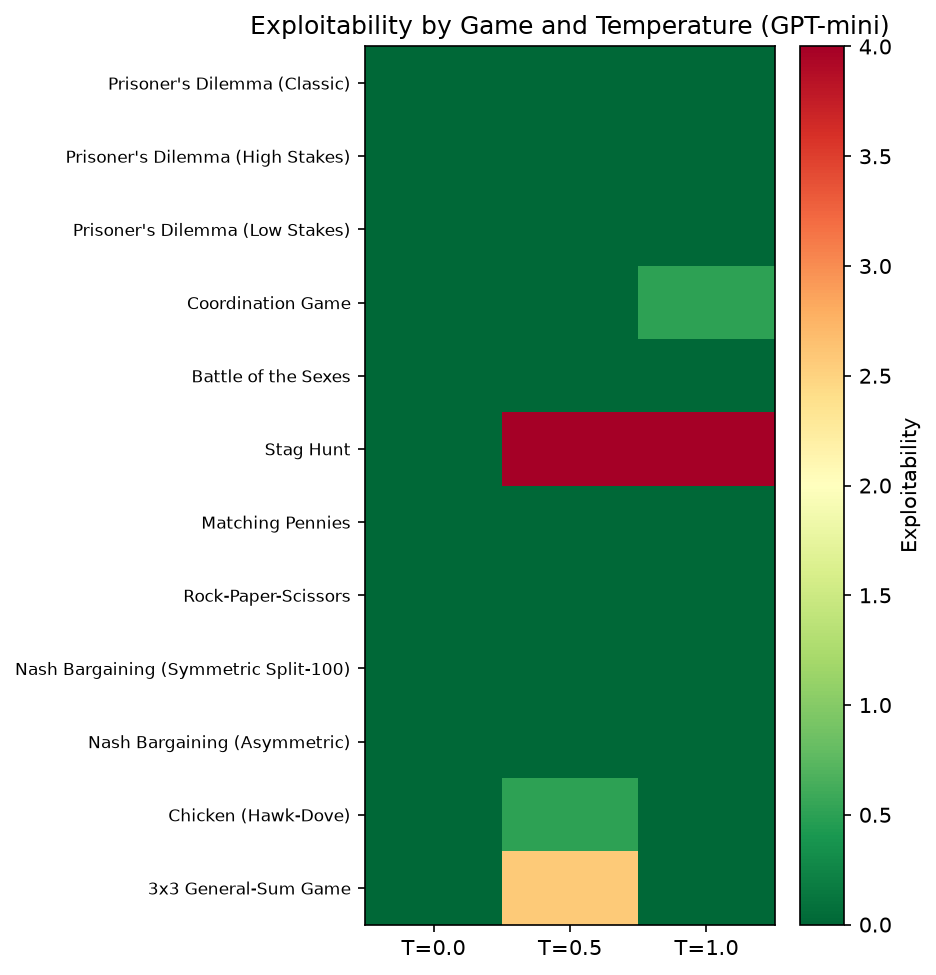
\includegraphics[width=\columnwidth]{../data/fig_heatmap_temp.png}
  \caption{Exploitability heatmap (GPT-mini). Darker red = more exploitable.}
  \label{fig:heatmap}
\end{figure}

\begin{figure}[h]
  \centering
  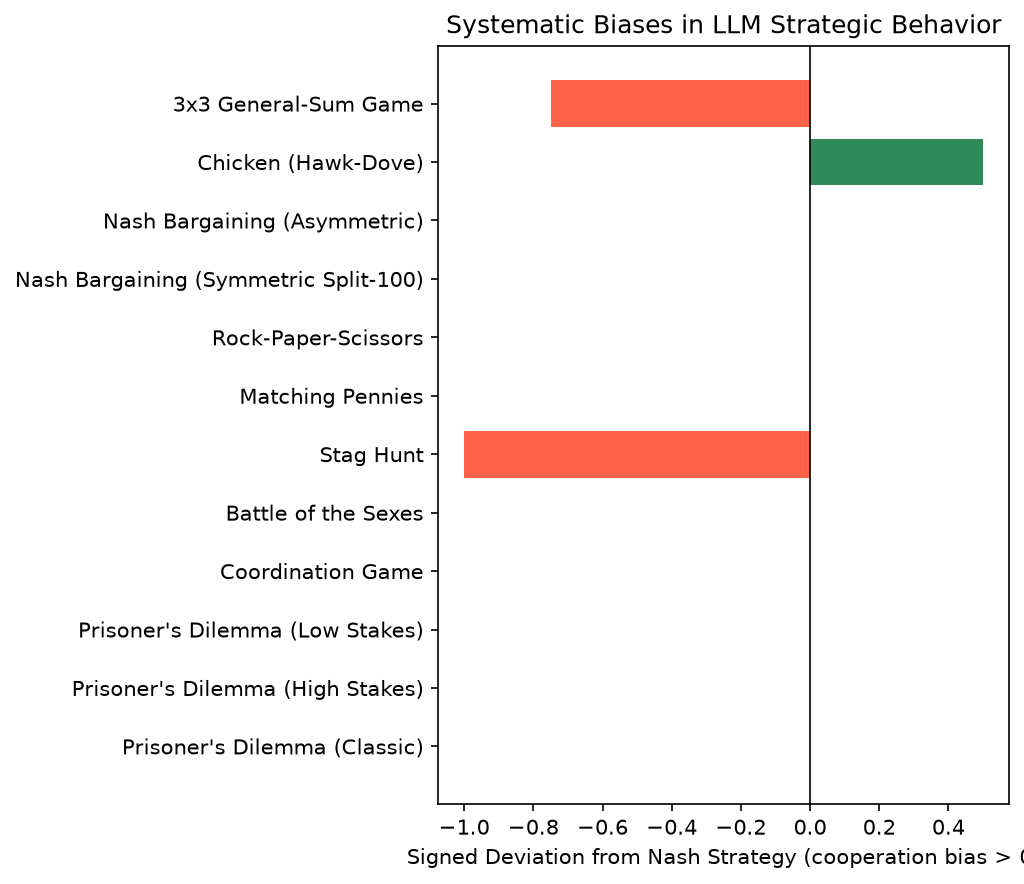
\includegraphics[width=\columnwidth]{../data/fig_bias.png}
  \caption{Signed deviation of LLM strategy from NE on the first action ($T{=}0.5$).
           Positive = plays first action more than Nash; negative = less.}
  \label{fig:bias}
\end{figure}

\subsection{Model Comparison ($T = 1$)}

\begin{table}[h]
\centering
\small
\begin{tabular}{lc}
\toprule
\textbf{Model} & \textbf{Mean } $\varepsilon$ \\
\midrule
GPT-5-mini          & \quad \\
Claude Haiku 4.5    & \quad \\
Claude Sonnet 4.5   & \quad \\
\bottomrule
\end{tabular}
\caption{Mean exploitability across all 12 games at $T{=}1$.}
\label{tab:models}
\end{table}

%% ─────────────────────────────────────────────
\section{Discussion}
%% ─────────────────────────────────────────────

\subsection{Cooperation Bias in Social Dilemmas}

In the Prisoner's Dilemma, Defect strictly dominates Cooperate regardless of
the opponent's action: $u_1(\text{D}, \cdot) > u_1(\text{C}, \cdot)$ for any
opponent strategy.
Iterated elimination of dominated strategies immediately yields (D, D) as the
unique NE.
Despite this, prior work has shown that LLMs frequently choose Cooperate, a
phenomenon termed \emph{cooperation bias}~\cite{akata2023repeated}.

% FILL IN: Did you observe this? Did payoff scale affect it (classic vs high/low)?
% Example: "Across all three PD variants, GPT-mini cooperated in X% of trials
%           at T=0, well above the NE prediction of 0%.
%           Cooperation rates were similar across payoff scales..."

\subsection{Failure to Randomize in Zero-Sum Games}

In zero-sum games, the unique NE requires uniform randomization: any
non-uniform strategy is exploitable by an opponent who best-responds to
the empirical frequencies~\cite{vonneumann1928}.
For Matching Pennies the NE is $(0.5, 0.5)$ over Heads/Tails; for
Rock-Paper-Scissors it is $(1/3, 1/3, 1/3)$.

% FILL IN: Did the LLM randomize uniformly? Was there a rock/heads bias?
% Example: "GPT-mini played Heads with probability X at T=0, well above the
%           NE prediction of 0.5. This translates to exploitability of Y..."

A deterministic bias is especially damaging in zero-sum games because an
adversary who knows the LLM's tendency can earn strictly positive expected
payoff indefinitely.

\subsection{Focal-Point Effects in Coordination Games}

When multiple Nash equilibria exist, game theory alone cannot select among
them~\cite{nash1950equilibrium}.
Schelling~\cite{schelling1960} argued that players often converge on
\emph{focal points}---salient options that stand out by convention or
presentation order.

% FILL IN: Did the LLM show a bias toward the first-listed action?
% In the Stag Hunt, did it prefer Pareto-optimal (Stag,Stag) or risk-dominant (Hare,Hare)?

In the Stag Hunt, both (Stag, Stag)---the Pareto-optimal equilibrium---and
(Hare, Hare)---the risk-dominant equilibrium---are Nash equilibria.
The course framework (Lecture 4) distinguishes these by Pareto efficiency and
risk dominance; LLM behavior here reveals which selection criterion the model
implicitly applies.

\subsection{Equality Bias in Bargaining}

The Nash Bargaining Solution (NBS) maximizes the Nash product
$\prod_i (u_i - d_i)$ over the feasible set, where $d_i$ is player $i$'s
disagreement payoff~\cite{nash1950bargaining}.
In the asymmetric variant (Row's outside option = 30, Col's = 10, surplus = 100),
the NBS assigns Row a payoff of 60 and Col a payoff of 40.
An LLM exhibiting \emph{equality bias} would instead demand 50,
deviating from the NBS by ignoring the asymmetry in outside options.

% FILL IN: Did the LLM demand 50 in the asymmetric game?
% This would show equality bias overriding rational bargaining.

\subsection{Effect of Temperature}

% FILL IN: Did exploitability increase or decrease with temperature?
% Higher temperature -> more random outputs -> closer to uniform mix -> could
% accidentally be closer to mixed NE in zero-sum games but further from pure NE in PD.

From the regret-minimization perspective (Lectures~7--9), temperature is not
equivalent to a regret-minimizing update.
A no-regret learner converges to Nash by systematically shifting weight toward
better-performing actions; temperature merely scales the output distribution
without responding to payoff feedback.

\subsection{Model Comparison}

% FILL IN: Did Claude Sonnet outperform GPT-mini? Did Haiku's lack of
% extended thinking hurt or help?

\subsection{Limitations}

\textbf{Prompt sensitivity.}
LLM responses may vary with prompt wording; we use a standardized prompt but
do not test paraphrases.
\textbf{Parsing noise.}
Responses that do not match any action clearly fall back to uniform
distributions, artificially reducing measured exploitability.
\textbf{Single-shot play.}
Strategic rationality may emerge differently in repeated interaction;
we test only one-shot decisions.
\textbf{Model opacity.}
We observe only final action choices, not the internal reasoning chain
that produced them.

%% ─────────────────────────────────────────────
\section*{LLM Disclosure}
%% ─────────────────────────────────────────────
Claude (Anthropic) was used to assist with code scaffolding, debugging, and
initial report structure. All experimental design, analysis, interpretation,
and final writing are my own. I am prepared to explain every part of the
submitted code and analysis.

%% ─────────────────────────────────────────────
\begin{thebibliography}{9}

\bibitem{nash1950equilibrium}
Nash, J.~F. (1950).
Equilibrium points in $n$-person games.
\textit{Proceedings of the National Academy of Sciences}, 36(1), 48--49.

\bibitem{nash1950bargaining}
Nash, J.~F. (1950).
The bargaining problem.
\textit{Econometrica}, 18(2), 155--162.

\bibitem{vonneumann1928}
von Neumann, J. (1928).
Zur Theorie der Gesellschaftsspiele.
\textit{Mathematische Annalen}, 100, 295--320.

\bibitem{schelling1960}
Schelling, T.~C. (1960).
\textit{The Strategy of Conflict}.
Harvard University Press.

\bibitem{akata2023repeated}
Akata, E., Schulz, L., Coda-Forno, J., Oh, S.~J., Bethge, M., \& Schulz, E. (2023).
Playing repeated games with large language models.
\textit{arXiv preprint arXiv:2305.16867}.

\bibitem{zinkevich2007}
Zinkevich, M., Johanson, M., Bowling, M., \& Piccione, C. (2007).
Regret minimization in games with incomplete information.
\textit{Advances in Neural Information Processing Systems}, 20.

\bibitem{nisan2007}
Nisan, N., Roughgarden, T., Tardos, E., \& Vazirani, V.~V. (Eds.) (2007).
\textit{Algorithmic Game Theory}.
Cambridge University Press.

\bibitem{nashpy}
Knight, V. \& Campbell, J. (2018).
Nashpy: A Python library for the computation of Nash equilibria.
\texttt{github.com/drvinceknight/Nashpy}.

\end{thebibliography}
%% ─────────────────────────────────────────────

\end{document}
